% !TEX encoding = UTF-8 Unicode
\documentclass[10pt]{standalone}\usepackage{tikz,graphicx}
\usepackage{fontspec}
\setmainfont{Arial}
\setsansfont{Arial}\begin{document}

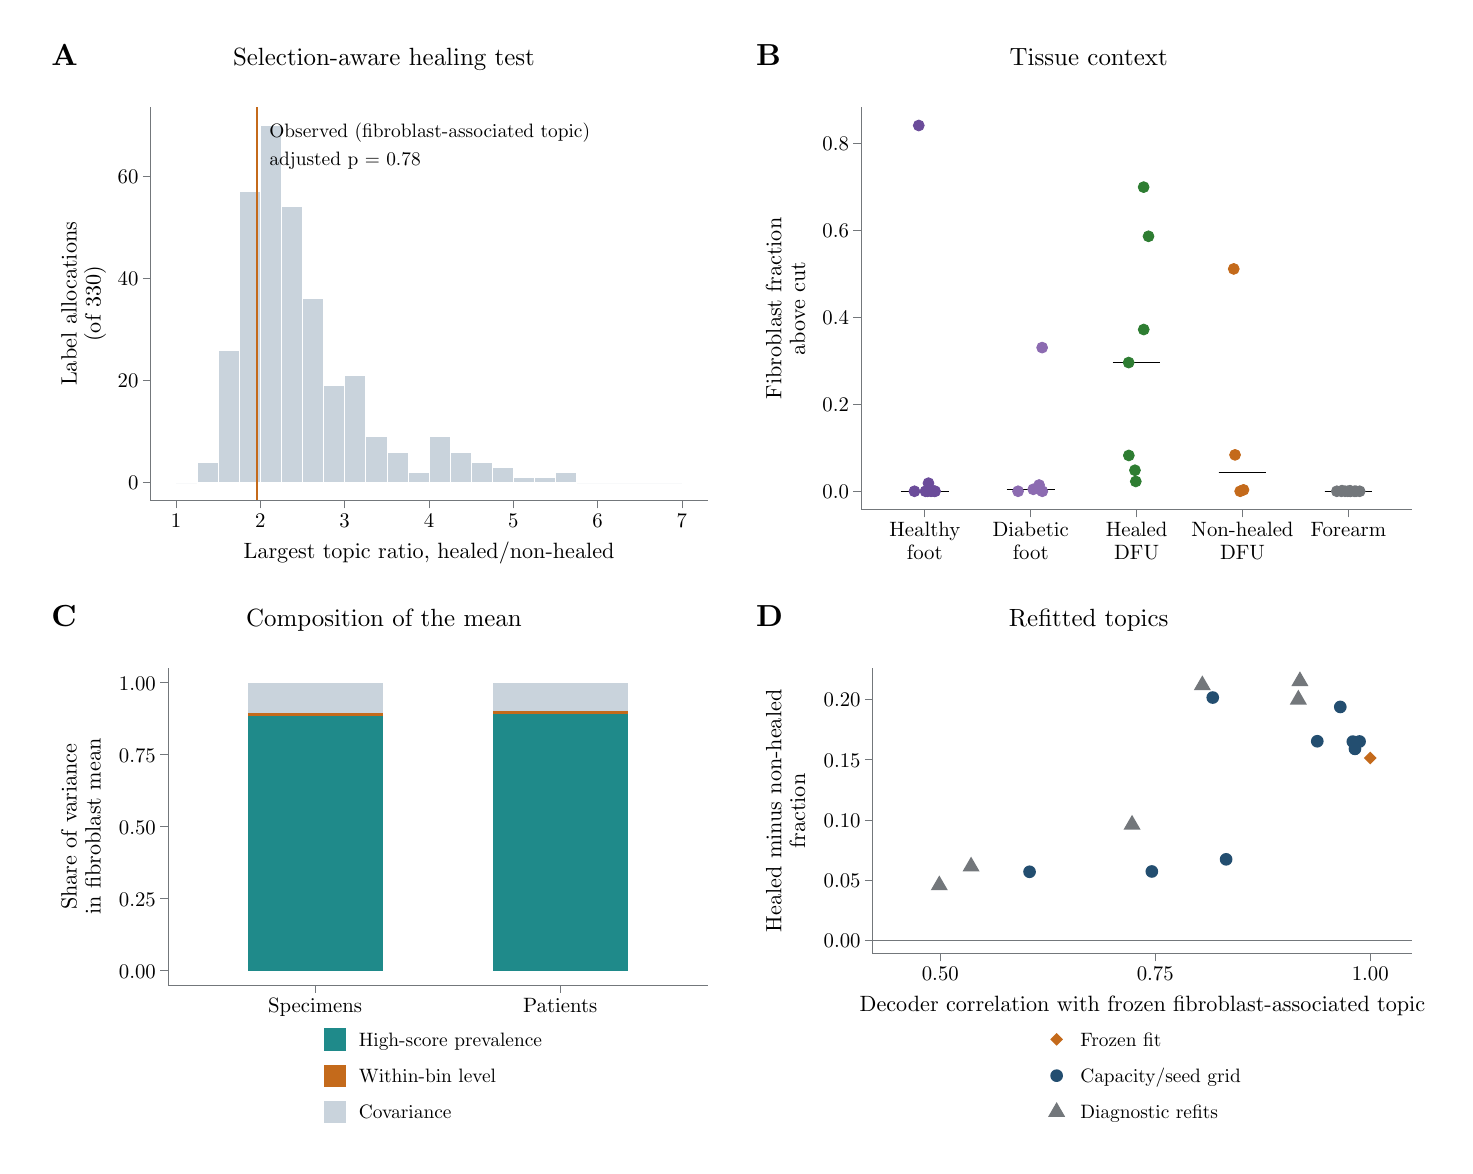
\begin{tikzpicture}[x=1pt,y=1pt]
\definecolor{fillColor}{RGB}{255,255,255}
\path[use as bounding box,fill=fillColor,fill opacity=0.00] (0,0) rectangle (512.15,404.03);
\begin{scope}
\path[clip] (  0.00,  0.00) rectangle (512.15,404.03);
\definecolor{drawColor}{RGB}{0,0,0}

\node[text=drawColor,anchor=base west,inner sep=0pt, outer sep=0pt, scale=  1.10] at (  8.54,390.46) {\bfseries A};

\node[text=drawColor,anchor=base,inner sep=0pt, outer sep=0pt, scale=  0.90] at (128.75,390.47) {Selection-aware healing test};
\end{scope}
\begin{scope}
\path[clip] (  8.54,206.99) rectangle (248.96,380.41);
\definecolor{fillColor}{RGB}{255,255,255}

\path[fill=fillColor] (  8.54,206.99) rectangle (248.96,380.41);
\end{scope}
\begin{scope}
\path[clip] ( 44.49,233.19) rectangle (245.55,375.29);
\definecolor{fillColor}{RGB}{255,255,255}

\path[fill=fillColor] ( 44.49,233.19) rectangle (245.55,375.29);
\definecolor{drawColor}{RGB}{255,255,255}
\definecolor{fillColor}{RGB}{201,211,220}

\path[draw=drawColor,line width= 0.2pt,fill=fillColor] ( 53.63,239.65) rectangle ( 61.24,239.65);

\path[draw=drawColor,line width= 0.2pt,fill=fillColor] ( 61.24,239.65) rectangle ( 68.86,247.03);

\path[draw=drawColor,line width= 0.2pt,fill=fillColor] ( 68.86,239.65) rectangle ( 76.47,287.63);

\path[draw=drawColor,line width= 0.2pt,fill=fillColor] ( 76.47,239.65) rectangle ( 84.09,344.84);

\path[draw=drawColor,line width= 0.2pt,fill=fillColor] ( 84.09,239.65) rectangle ( 91.71,368.83);

\path[draw=drawColor,line width= 0.2pt,fill=fillColor] ( 91.71,239.65) rectangle ( 99.32,339.31);

\path[draw=drawColor,line width= 0.2pt,fill=fillColor] ( 99.32,239.65) rectangle (106.94,306.09);

\path[draw=drawColor,line width= 0.2pt,fill=fillColor] (106.94,239.65) rectangle (114.55,274.72);

\path[draw=drawColor,line width= 0.2pt,fill=fillColor] (114.55,239.65) rectangle (122.17,278.41);

\path[draw=drawColor,line width= 0.2pt,fill=fillColor] (122.17,239.65) rectangle (129.79,256.26);

\path[draw=drawColor,line width= 0.2pt,fill=fillColor] (129.79,239.65) rectangle (137.40,250.73);

\path[draw=drawColor,line width= 0.2pt,fill=fillColor] (137.40,239.65) rectangle (145.02,243.34);

\path[draw=drawColor,line width= 0.2pt,fill=fillColor] (145.02,239.65) rectangle (152.63,256.26);

\path[draw=drawColor,line width= 0.2pt,fill=fillColor] (152.63,239.65) rectangle (160.25,250.73);

\path[draw=drawColor,line width= 0.2pt,fill=fillColor] (160.25,239.65) rectangle (167.86,247.03);

\path[draw=drawColor,line width= 0.2pt,fill=fillColor] (167.86,239.65) rectangle (175.48,245.19);

\path[draw=drawColor,line width= 0.2pt,fill=fillColor] (175.48,239.65) rectangle (183.10,241.50);

\path[draw=drawColor,line width= 0.2pt,fill=fillColor] (183.10,239.65) rectangle (190.71,241.50);

\path[draw=drawColor,line width= 0.2pt,fill=fillColor] (190.71,239.65) rectangle (198.33,243.34);

\path[draw=drawColor,line width= 0.2pt,fill=fillColor] (198.33,239.65) rectangle (205.94,239.65);

\path[draw=drawColor,line width= 0.2pt,fill=fillColor] (205.94,239.65) rectangle (213.56,239.65);

\path[draw=drawColor,line width= 0.2pt,fill=fillColor] (213.56,239.65) rectangle (221.18,239.65);

\path[draw=drawColor,line width= 0.2pt,fill=fillColor] (221.18,239.65) rectangle (228.79,239.65);

\path[draw=drawColor,line width= 0.2pt,fill=fillColor] (228.79,239.65) rectangle (236.41,239.65);
\definecolor{drawColor}{RGB}{196,106,27}

\path[draw=drawColor,line width= 0.7pt,line join=round] ( 82.78,233.19) -- ( 82.78,375.29);
\definecolor{drawColor}{RGB}{0,0,0}

\node[text=drawColor,anchor=base west,inner sep=0pt, outer sep=0pt, scale=  0.70] at ( 87.35,364.24) {Observed (fibroblast-associated topic)};

\node[text=drawColor,anchor=base west,inner sep=0pt, outer sep=0pt, scale=  0.70] at ( 87.35,354.16) {adjusted p = 0.78};
\end{scope}
\begin{scope}
\path[clip] (  0.00,  0.00) rectangle (512.15,404.03);
\definecolor{drawColor}{RGB}{115,119,123}

\path[draw=drawColor,line width= 0.3pt,line join=round,line cap=rect] ( 44.49,233.19) --
	( 44.49,375.29);
\end{scope}
\begin{scope}
\path[clip] (  0.00,  0.00) rectangle (512.15,404.03);
\definecolor{drawColor}{RGB}{0,0,0}

\node[text=drawColor,anchor=base east,inner sep=0pt, outer sep=0pt, scale=  0.75] at ( 40.04,236.97) {0};

\node[text=drawColor,anchor=base east,inner sep=0pt, outer sep=0pt, scale=  0.75] at ( 40.04,273.88) {20};

\node[text=drawColor,anchor=base east,inner sep=0pt, outer sep=0pt, scale=  0.75] at ( 40.04,310.79) {40};

\node[text=drawColor,anchor=base east,inner sep=0pt, outer sep=0pt, scale=  0.75] at ( 40.04,347.69) {60};
\end{scope}
\begin{scope}
\path[clip] (  0.00,  0.00) rectangle (512.15,404.03);
\definecolor{drawColor}{RGB}{115,119,123}

\path[draw=drawColor,line width= 0.3pt,line join=round] ( 41.64,239.65) --
	( 44.49,239.65);

\path[draw=drawColor,line width= 0.3pt,line join=round] ( 41.64,276.56) --
	( 44.49,276.56);

\path[draw=drawColor,line width= 0.3pt,line join=round] ( 41.64,313.47) --
	( 44.49,313.47);

\path[draw=drawColor,line width= 0.3pt,line join=round] ( 41.64,350.38) --
	( 44.49,350.38);
\end{scope}
\begin{scope}
\path[clip] (  0.00,  0.00) rectangle (512.15,404.03);
\definecolor{drawColor}{RGB}{115,119,123}

\path[draw=drawColor,line width= 0.3pt,line join=round,line cap=rect] ( 44.49,233.19) --
	(245.55,233.19);
\end{scope}
\begin{scope}
\path[clip] (  0.00,  0.00) rectangle (512.15,404.03);
\definecolor{drawColor}{RGB}{115,119,123}

\path[draw=drawColor,line width= 0.3pt,line join=round] ( 53.63,230.35) --
	( 53.63,233.19);

\path[draw=drawColor,line width= 0.3pt,line join=round] ( 84.09,230.35) --
	( 84.09,233.19);

\path[draw=drawColor,line width= 0.3pt,line join=round] (114.55,230.35) --
	(114.55,233.19);

\path[draw=drawColor,line width= 0.3pt,line join=round] (145.02,230.35) --
	(145.02,233.19);

\path[draw=drawColor,line width= 0.3pt,line join=round] (175.48,230.35) --
	(175.48,233.19);

\path[draw=drawColor,line width= 0.3pt,line join=round] (205.94,230.35) --
	(205.94,233.19);

\path[draw=drawColor,line width= 0.3pt,line join=round] (236.41,230.35) --
	(236.41,233.19);
\end{scope}
\begin{scope}
\path[clip] (  0.00,  0.00) rectangle (512.15,404.03);
\definecolor{drawColor}{RGB}{0,0,0}

\node[text=drawColor,anchor=base,inner sep=0pt, outer sep=0pt, scale=  0.75] at ( 53.63,223.38) {1};

\node[text=drawColor,anchor=base,inner sep=0pt, outer sep=0pt, scale=  0.75] at ( 84.09,223.38) {2};

\node[text=drawColor,anchor=base,inner sep=0pt, outer sep=0pt, scale=  0.75] at (114.55,223.38) {3};

\node[text=drawColor,anchor=base,inner sep=0pt, outer sep=0pt, scale=  0.75] at (145.02,223.38) {4};

\node[text=drawColor,anchor=base,inner sep=0pt, outer sep=0pt, scale=  0.75] at (175.48,223.38) {5};

\node[text=drawColor,anchor=base,inner sep=0pt, outer sep=0pt, scale=  0.75] at (205.94,223.38) {6};

\node[text=drawColor,anchor=base,inner sep=0pt, outer sep=0pt, scale=  0.75] at (236.41,223.38) {7};
\end{scope}
\begin{scope}
\path[clip] (  0.00,  0.00) rectangle (512.15,404.03);
\definecolor{drawColor}{RGB}{0,0,0}

\node[text=drawColor,anchor=base,inner sep=0pt, outer sep=0pt, scale=  0.80] at (145.02,212.09) {Largest topic ratio, healed/non-healed};
\end{scope}
\begin{scope}
\path[clip] (  0.00,  0.00) rectangle (512.15,404.03);
\definecolor{drawColor}{RGB}{0,0,0}

\node[text=drawColor,rotate= 90.00,anchor=base,inner sep=0pt, outer sep=0pt, scale=  0.80] at ( 17.68,304.24) {Label allocations};

\node[text=drawColor,rotate= 90.00,anchor=base,inner sep=0pt, outer sep=0pt, scale=  0.80] at ( 26.32,304.24) {(of 330)};
\end{scope}
\begin{scope}
\path[clip] (  0.00,  0.00) rectangle (512.15,404.03);
\definecolor{drawColor}{RGB}{0,0,0}

\node[text=drawColor,anchor=base west,inner sep=0pt, outer sep=0pt, scale=  1.10] at (263.19,390.46) {\bfseries B};

\node[text=drawColor,anchor=base,inner sep=0pt, outer sep=0pt, scale=  0.90] at (383.40,390.47) {Tissue context};
\end{scope}
\begin{scope}
\path[clip] (263.19,206.99) rectangle (503.61,380.41);
\definecolor{fillColor}{RGB}{255,255,255}

\path[fill=fillColor] (263.19,206.99) rectangle (503.61,380.41);
\end{scope}
\begin{scope}
\path[clip] (301.22,229.90) rectangle (500.20,375.29);
\definecolor{fillColor}{RGB}{255,255,255}

\path[fill=fillColor] (301.22,229.90) rectangle (500.20,375.29);
\definecolor{drawColor}{RGB}{0,0,0}

\path[draw=drawColor,line width= 0.4pt,line join=round] (315.57,236.51) --
	(332.79,236.51);

\path[draw=drawColor,line width= 0.4pt,line join=round] (324.18,236.51) --
	(324.18,236.51);

\path[draw=drawColor,line width= 0.4pt,line join=round] (315.57,236.51) --
	(332.79,236.51);

\path[draw=drawColor,line width= 0.4pt,line join=round] (353.84,237.23) --
	(371.06,237.23);

\path[draw=drawColor,line width= 0.4pt,line join=round] (362.45,237.23) --
	(362.45,237.23);

\path[draw=drawColor,line width= 0.4pt,line join=round] (353.84,237.23) --
	(371.06,237.23);

\path[draw=drawColor,line width= 0.4pt,line join=round] (392.10,283.01) --
	(409.32,283.01);

\path[draw=drawColor,line width= 0.4pt,line join=round] (400.71,283.01) --
	(400.71,283.01);

\path[draw=drawColor,line width= 0.4pt,line join=round] (392.10,283.01) --
	(409.32,283.01);

\path[draw=drawColor,line width= 0.4pt,line join=round] (430.37,243.34) --
	(447.59,243.34);

\path[draw=drawColor,line width= 0.4pt,line join=round] (438.98,243.34) --
	(438.98,243.34);

\path[draw=drawColor,line width= 0.4pt,line join=round] (430.37,243.34) --
	(447.59,243.34);

\path[draw=drawColor,line width= 0.4pt,line join=round] (468.63,236.51) --
	(485.85,236.51);

\path[draw=drawColor,line width= 0.4pt,line join=round] (477.24,236.51) --
	(477.24,236.51);

\path[draw=drawColor,line width= 0.4pt,line join=round] (468.63,236.51) --
	(485.85,236.51);
\definecolor{drawColor}{RGB}{196,106,27}
\definecolor{fillColor}{RGB}{196,106,27}

\path[draw=drawColor,line width= 0.3pt,line join=round,line cap=round,fill=fillColor] (435.81,316.85) circle (  1.97);
\definecolor{drawColor}{RGB}{46,125,50}
\definecolor{fillColor}{RGB}{46,125,50}

\path[draw=drawColor,line width= 0.3pt,line join=round,line cap=round,fill=fillColor] (405.01,328.64) circle (  1.97);

\path[draw=drawColor,line width= 0.3pt,line join=round,line cap=round,fill=fillColor] (400.42,240.06) circle (  1.97);

\path[draw=drawColor,line width= 0.3pt,line join=round,line cap=round,fill=fillColor] (403.25,346.41) circle (  1.97);
\definecolor{drawColor}{RGB}{196,106,27}
\definecolor{fillColor}{RGB}{196,106,27}

\path[draw=drawColor,line width= 0.3pt,line join=round,line cap=round,fill=fillColor] (438.13,236.51) circle (  1.97);

\path[draw=drawColor,line width= 0.3pt,line join=round,line cap=round,fill=fillColor] (439.33,237.02) circle (  1.97);

\path[draw=drawColor,line width= 0.3pt,line join=round,line cap=round,fill=fillColor] (436.28,249.66) circle (  1.97);
\definecolor{drawColor}{RGB}{46,125,50}
\definecolor{fillColor}{RGB}{46,125,50}

\path[draw=drawColor,line width= 0.3pt,line join=round,line cap=round,fill=fillColor] (397.84,283.01) circle (  1.97);

\path[draw=drawColor,line width= 0.3pt,line join=round,line cap=round,fill=fillColor] (403.28,294.95) circle (  1.97);

\path[draw=drawColor,line width= 0.3pt,line join=round,line cap=round,fill=fillColor] (397.90,249.45) circle (  1.97);

\path[draw=drawColor,line width= 0.3pt,line join=round,line cap=round,fill=fillColor] (400.11,244.10) circle (  1.97);
\definecolor{drawColor}{RGB}{140,107,177}
\definecolor{fillColor}{RGB}{140,107,177}

\path[draw=drawColor,line width= 0.3pt,line join=round,line cap=round,fill=fillColor] (357.88,236.51) circle (  1.97);

\path[draw=drawColor,line width= 0.3pt,line join=round,line cap=round,fill=fillColor] (365.52,237.25) circle (  1.97);

\path[draw=drawColor,line width= 0.3pt,line join=round,line cap=round,fill=fillColor] (365.48,238.76) circle (  1.97);

\path[draw=drawColor,line width= 0.3pt,line join=round,line cap=round,fill=fillColor] (366.64,236.51) circle (  1.97);

\path[draw=drawColor,line width= 0.3pt,line join=round,line cap=round,fill=fillColor] (366.57,288.42) circle (  1.97);

\path[draw=drawColor,line width= 0.3pt,line join=round,line cap=round,fill=fillColor] (363.37,237.21) circle (  1.97);
\definecolor{drawColor}{RGB}{107,76,154}
\definecolor{fillColor}{RGB}{107,76,154}

\path[draw=drawColor,line width= 0.3pt,line join=round,line cap=round,fill=fillColor] (321.99,368.68) circle (  1.97);

\path[draw=drawColor,line width= 0.3pt,line join=round,line cap=round,fill=fillColor] (325.50,239.43) circle (  1.97);

\path[draw=drawColor,line width= 0.3pt,line join=round,line cap=round,fill=fillColor] (324.42,236.51) circle (  1.97);

\path[draw=drawColor,line width= 0.3pt,line join=round,line cap=round,fill=fillColor] (327.68,236.51) circle (  1.97);

\path[draw=drawColor,line width= 0.3pt,line join=round,line cap=round,fill=fillColor] (325.17,236.51) circle (  1.97);

\path[draw=drawColor,line width= 0.3pt,line join=round,line cap=round,fill=fillColor] (326.39,236.51) circle (  1.97);

\path[draw=drawColor,line width= 0.3pt,line join=round,line cap=round,fill=fillColor] (326.97,236.67) circle (  1.97);

\path[draw=drawColor,line width= 0.3pt,line join=round,line cap=round,fill=fillColor] (327.88,236.51) circle (  1.97);

\path[draw=drawColor,line width= 0.3pt,line join=round,line cap=round,fill=fillColor] (320.44,236.51) circle (  1.97);
\definecolor{drawColor}{RGB}{115,119,123}
\definecolor{fillColor}{RGB}{115,119,123}

\path[draw=drawColor,line width= 0.3pt,line join=round,line cap=round,fill=fillColor] (477.93,236.51) circle (  1.97);

\path[draw=drawColor,line width= 0.3pt,line join=round,line cap=round,fill=fillColor] (477.93,236.51) circle (  1.97);

\path[draw=drawColor,line width= 0.3pt,line join=round,line cap=round,fill=fillColor] (481.32,236.51) circle (  1.97);

\path[draw=drawColor,line width= 0.3pt,line join=round,line cap=round,fill=fillColor] (474.66,236.51) circle (  1.97);

\path[draw=drawColor,line width= 0.3pt,line join=round,line cap=round,fill=fillColor] (477.04,236.51) circle (  1.97);

\path[draw=drawColor,line width= 0.3pt,line join=round,line cap=round,fill=fillColor] (473.06,236.51) circle (  1.97);

\path[draw=drawColor,line width= 0.3pt,line join=round,line cap=round,fill=fillColor] (479.99,236.51) circle (  1.97);

\path[draw=drawColor,line width= 0.3pt,line join=round,line cap=round,fill=fillColor] (476.03,236.51) circle (  1.97);

\path[draw=drawColor,line width= 0.3pt,line join=round,line cap=round,fill=fillColor] (477.82,236.69) circle (  1.97);

\path[draw=drawColor,line width= 0.3pt,line join=round,line cap=round,fill=fillColor] (474.92,236.73) circle (  1.97);

\path[draw=drawColor,line width= 0.3pt,line join=round,line cap=round,fill=fillColor] (479.39,236.51) circle (  1.97);
\end{scope}
\begin{scope}
\path[clip] (  0.00,  0.00) rectangle (512.15,404.03);
\definecolor{drawColor}{RGB}{115,119,123}

\path[draw=drawColor,line width= 0.3pt,line join=round,line cap=rect] (301.22,229.90) --
	(301.22,375.29);
\end{scope}
\begin{scope}
\path[clip] (  0.00,  0.00) rectangle (512.15,404.03);
\definecolor{drawColor}{RGB}{0,0,0}

\node[text=drawColor,anchor=base east,inner sep=0pt, outer sep=0pt, scale=  0.75] at (296.78,233.82) {0.0};

\node[text=drawColor,anchor=base east,inner sep=0pt, outer sep=0pt, scale=  0.75] at (296.78,265.25) {0.2};

\node[text=drawColor,anchor=base east,inner sep=0pt, outer sep=0pt, scale=  0.75] at (296.78,296.68) {0.4};

\node[text=drawColor,anchor=base east,inner sep=0pt, outer sep=0pt, scale=  0.75] at (296.78,328.10) {0.6};

\node[text=drawColor,anchor=base east,inner sep=0pt, outer sep=0pt, scale=  0.75] at (296.78,359.53) {0.8};
\end{scope}
\begin{scope}
\path[clip] (  0.00,  0.00) rectangle (512.15,404.03);
\definecolor{drawColor}{RGB}{115,119,123}

\path[draw=drawColor,line width= 0.3pt,line join=round] (298.38,236.51) --
	(301.22,236.51);

\path[draw=drawColor,line width= 0.3pt,line join=round] (298.38,267.94) --
	(301.22,267.94);

\path[draw=drawColor,line width= 0.3pt,line join=round] (298.38,299.36) --
	(301.22,299.36);

\path[draw=drawColor,line width= 0.3pt,line join=round] (298.38,330.79) --
	(301.22,330.79);

\path[draw=drawColor,line width= 0.3pt,line join=round] (298.38,362.21) --
	(301.22,362.21);
\end{scope}
\begin{scope}
\path[clip] (  0.00,  0.00) rectangle (512.15,404.03);
\definecolor{drawColor}{RGB}{115,119,123}

\path[draw=drawColor,line width= 0.3pt,line join=round,line cap=rect] (301.22,229.90) --
	(500.20,229.90);
\end{scope}
\begin{scope}
\path[clip] (  0.00,  0.00) rectangle (512.15,404.03);
\definecolor{drawColor}{RGB}{115,119,123}

\path[draw=drawColor,line width= 0.3pt,line join=round] (324.18,227.06) --
	(324.18,229.90);

\path[draw=drawColor,line width= 0.3pt,line join=round] (362.45,227.06) --
	(362.45,229.90);

\path[draw=drawColor,line width= 0.3pt,line join=round] (400.71,227.06) --
	(400.71,229.90);

\path[draw=drawColor,line width= 0.3pt,line join=round] (438.98,227.06) --
	(438.98,229.90);

\path[draw=drawColor,line width= 0.3pt,line join=round] (477.24,227.06) --
	(477.24,229.90);
\end{scope}
\begin{scope}
\path[clip] (  0.00,  0.00) rectangle (512.15,404.03);
\definecolor{drawColor}{RGB}{0,0,0}

\node[text=drawColor,anchor=base,inner sep=0pt, outer sep=0pt, scale=  0.75] at (324.18,220.09) {Healthy};

\node[text=drawColor,anchor=base,inner sep=0pt, outer sep=0pt, scale=  0.75] at (324.18,211.99) {foot};

\node[text=drawColor,anchor=base,inner sep=0pt, outer sep=0pt, scale=  0.75] at (362.45,220.09) {Diabetic};

\node[text=drawColor,anchor=base,inner sep=0pt, outer sep=0pt, scale=  0.75] at (362.45,211.99) {foot};

\node[text=drawColor,anchor=base,inner sep=0pt, outer sep=0pt, scale=  0.75] at (400.71,220.09) {Healed};

\node[text=drawColor,anchor=base,inner sep=0pt, outer sep=0pt, scale=  0.75] at (400.71,211.99) {DFU};

\node[text=drawColor,anchor=base,inner sep=0pt, outer sep=0pt, scale=  0.75] at (438.98,220.09) {Non-healed};

\node[text=drawColor,anchor=base,inner sep=0pt, outer sep=0pt, scale=  0.75] at (438.98,211.99) {DFU};

\node[text=drawColor,anchor=base,inner sep=0pt, outer sep=0pt, scale=  0.75] at (477.24,220.09) {Forearm};
\end{scope}
\begin{scope}
\path[clip] (  0.00,  0.00) rectangle (512.15,404.03);
\definecolor{drawColor}{RGB}{0,0,0}

\node[text=drawColor,rotate= 90.00,anchor=base,inner sep=0pt, outer sep=0pt, scale=  0.80] at (272.33,302.60) {Fibroblast fraction};

\node[text=drawColor,rotate= 90.00,anchor=base,inner sep=0pt, outer sep=0pt, scale=  0.80] at (280.97,302.60) {above cut};
\end{scope}
\begin{scope}
\path[clip] (  0.00,  0.00) rectangle (512.15,404.03);
\definecolor{drawColor}{RGB}{0,0,0}

\node[text=drawColor,anchor=base west,inner sep=0pt, outer sep=0pt, scale=  1.10] at (  8.54,187.74) {\bfseries C};

\node[text=drawColor,anchor=base,inner sep=0pt, outer sep=0pt, scale=  0.90] at (128.75,187.75) {Composition of the mean};
\end{scope}
\begin{scope}
\path[clip] (  8.54,  4.27) rectangle (248.96,177.69);
\definecolor{fillColor}{RGB}{255,255,255}

\path[fill=fillColor] (  8.54,  4.27) rectangle (248.96,177.69);
\end{scope}
\begin{scope}
\path[clip] ( 50.74, 58.09) rectangle (245.55,172.57);
\definecolor{fillColor}{RGB}{255,255,255}

\path[fill=fillColor] ( 50.74, 58.09) rectangle (245.55,172.57);
\definecolor{fillColor}{RGB}{31,138,138}

\path[fill=fillColor] ( 79.52, 63.29) rectangle (128.22,155.29);
\definecolor{fillColor}{RGB}{196,106,27}

\path[fill=fillColor] ( 79.52,155.29) rectangle (128.22,156.49);
\definecolor{fillColor}{RGB}{201,211,220}

\path[fill=fillColor] ( 79.52,156.49) rectangle (128.22,167.36);
\definecolor{fillColor}{RGB}{31,138,138}

\path[fill=fillColor] (168.07, 63.29) rectangle (216.77,155.98);
\definecolor{fillColor}{RGB}{196,106,27}

\path[fill=fillColor] (168.07,155.98) rectangle (216.77,157.06);
\definecolor{fillColor}{RGB}{201,211,220}

\path[fill=fillColor] (168.07,157.06) rectangle (216.77,167.36);
\end{scope}
\begin{scope}
\path[clip] (  0.00,  0.00) rectangle (512.15,404.03);
\definecolor{drawColor}{RGB}{115,119,123}

\path[draw=drawColor,line width= 0.3pt,line join=round,line cap=rect] ( 50.74, 58.09) --
	( 50.74,172.57);
\end{scope}
\begin{scope}
\path[clip] (  0.00,  0.00) rectangle (512.15,404.03);
\definecolor{drawColor}{RGB}{0,0,0}

\node[text=drawColor,anchor=base east,inner sep=0pt, outer sep=0pt, scale=  0.75] at ( 46.30, 60.61) {0.00};

\node[text=drawColor,anchor=base east,inner sep=0pt, outer sep=0pt, scale=  0.75] at ( 46.30, 86.62) {0.25};

\node[text=drawColor,anchor=base east,inner sep=0pt, outer sep=0pt, scale=  0.75] at ( 46.30,112.64) {0.50};

\node[text=drawColor,anchor=base east,inner sep=0pt, outer sep=0pt, scale=  0.75] at ( 46.30,138.66) {0.75};

\node[text=drawColor,anchor=base east,inner sep=0pt, outer sep=0pt, scale=  0.75] at ( 46.30,164.68) {1.00};
\end{scope}
\begin{scope}
\path[clip] (  0.00,  0.00) rectangle (512.15,404.03);
\definecolor{drawColor}{RGB}{115,119,123}

\path[draw=drawColor,line width= 0.3pt,line join=round] ( 47.90, 63.29) --
	( 50.74, 63.29);

\path[draw=drawColor,line width= 0.3pt,line join=round] ( 47.90, 89.31) --
	( 50.74, 89.31);

\path[draw=drawColor,line width= 0.3pt,line join=round] ( 47.90,115.33) --
	( 50.74,115.33);

\path[draw=drawColor,line width= 0.3pt,line join=round] ( 47.90,141.34) --
	( 50.74,141.34);

\path[draw=drawColor,line width= 0.3pt,line join=round] ( 47.90,167.36) --
	( 50.74,167.36);
\end{scope}
\begin{scope}
\path[clip] (  0.00,  0.00) rectangle (512.15,404.03);
\definecolor{drawColor}{RGB}{115,119,123}

\path[draw=drawColor,line width= 0.3pt,line join=round,line cap=rect] ( 50.74, 58.09) --
	(245.55, 58.09);
\end{scope}
\begin{scope}
\path[clip] (  0.00,  0.00) rectangle (512.15,404.03);
\definecolor{drawColor}{RGB}{115,119,123}

\path[draw=drawColor,line width= 0.3pt,line join=round] (103.87, 55.24) --
	(103.87, 58.09);

\path[draw=drawColor,line width= 0.3pt,line join=round] (192.42, 55.24) --
	(192.42, 58.09);
\end{scope}
\begin{scope}
\path[clip] (  0.00,  0.00) rectangle (512.15,404.03);
\definecolor{drawColor}{RGB}{0,0,0}

\node[text=drawColor,anchor=base,inner sep=0pt, outer sep=0pt, scale=  0.75] at (103.87, 48.27) {Specimens};

\node[text=drawColor,anchor=base,inner sep=0pt, outer sep=0pt, scale=  0.75] at (192.42, 48.27) {Patients};
\end{scope}
\begin{scope}
\path[clip] (  0.00,  0.00) rectangle (512.15,404.03);
\definecolor{drawColor}{RGB}{0,0,0}

\node[text=drawColor,rotate= 90.00,anchor=base,inner sep=0pt, outer sep=0pt, scale=  0.80] at ( 17.68,115.33) {Share of variance};

\node[text=drawColor,rotate= 90.00,anchor=base,inner sep=0pt, outer sep=0pt, scale=  0.80] at ( 26.32,115.33) {in fibroblast mean};
\end{scope}
\begin{scope}
\path[clip] (  0.00,  0.00) rectangle (512.15,404.03);
\definecolor{fillColor}{RGB}{255,255,255}

\path[fill=fillColor] (106.58,  7.68) rectangle (189.71, 43.00);
\end{scope}
\begin{scope}
\path[clip] (  0.00,  0.00) rectangle (512.15,404.03);
\definecolor{fillColor}{RGB}{255,255,255}

\path[fill=fillColor] (106.58, 33.89) rectangle (115.68, 43.00);
\definecolor{fillColor}{RGB}{31,138,138}

\path[fill=fillColor] (107.09, 34.41) rectangle (115.16, 42.48);
\end{scope}
\begin{scope}
\path[clip] (  0.00,  0.00) rectangle (512.15,404.03);
\definecolor{fillColor}{RGB}{255,255,255}

\path[fill=fillColor] (106.58, 20.79) rectangle (115.68, 29.89);
\definecolor{fillColor}{RGB}{196,106,27}

\path[fill=fillColor] (107.09, 21.30) rectangle (115.16, 29.37);
\end{scope}
\begin{scope}
\path[clip] (  0.00,  0.00) rectangle (512.15,404.03);
\definecolor{fillColor}{RGB}{255,255,255}

\path[fill=fillColor] (106.58,  7.68) rectangle (115.68, 16.79);
\definecolor{fillColor}{RGB}{201,211,220}

\path[fill=fillColor] (107.09,  8.20) rectangle (115.16, 16.27);
\end{scope}
\begin{scope}
\path[clip] (  0.00,  0.00) rectangle (512.15,404.03);
\definecolor{drawColor}{RGB}{0,0,0}

\node[text=drawColor,anchor=base west,inner sep=0pt, outer sep=0pt, scale=  0.70] at (119.68, 35.94) {High-score prevalence};
\end{scope}
\begin{scope}
\path[clip] (  0.00,  0.00) rectangle (512.15,404.03);
\definecolor{drawColor}{RGB}{0,0,0}

\node[text=drawColor,anchor=base west,inner sep=0pt, outer sep=0pt, scale=  0.70] at (119.68, 22.83) {Within-bin level};
\end{scope}
\begin{scope}
\path[clip] (  0.00,  0.00) rectangle (512.15,404.03);
\definecolor{drawColor}{RGB}{0,0,0}

\node[text=drawColor,anchor=base west,inner sep=0pt, outer sep=0pt, scale=  0.70] at (119.68,  9.73) {Covariance};
\end{scope}
\begin{scope}
\path[clip] (  0.00,  0.00) rectangle (512.15,404.03);
\definecolor{drawColor}{RGB}{0,0,0}

\node[text=drawColor,anchor=base west,inner sep=0pt, outer sep=0pt, scale=  1.10] at (263.19,187.74) {\bfseries D};

\node[text=drawColor,anchor=base,inner sep=0pt, outer sep=0pt, scale=  0.90] at (383.40,187.75) {Refitted topics};
\end{scope}
\begin{scope}
\path[clip] (263.19,  4.27) rectangle (503.61,177.69);
\definecolor{fillColor}{RGB}{255,255,255}

\path[fill=fillColor] (263.19,  4.27) rectangle (503.61,177.69);
\end{scope}
\begin{scope}
\path[clip] (305.39, 69.48) rectangle (500.20,172.57);
\definecolor{fillColor}{RGB}{255,255,255}

\path[fill=fillColor] (305.39, 69.48) rectangle (500.20,172.57);
\definecolor{drawColor}{RGB}{115,119,123}

\path[draw=drawColor,line width= 0.3pt,line join=round] (305.39, 74.17) -- (500.20, 74.17);
\definecolor{fillColor}{RGB}{196,106,27}

\path[fill=fillColor] (482.84,140.14) --
	(485.13,142.43) --
	(487.42,140.14) --
	(485.13,137.84) --
	cycle;
\definecolor{fillColor}{RGB}{35,78,112}

\path[fill=fillColor] (428.22,161.97) circle (  2.29);

\path[fill=fillColor] (465.99,146.18) circle (  2.29);

\path[fill=fillColor] (474.31,158.58) circle (  2.29);

\path[fill=fillColor] (478.84,146.05) circle (  2.29);

\path[fill=fillColor] (479.61,143.42) circle (  2.29);

\path[fill=fillColor] (406.21, 99.12) circle (  2.29);

\path[fill=fillColor] (481.28,146.10) circle (  2.29);

\path[fill=fillColor] (433.05,103.51) circle (  2.29);

\path[fill=fillColor] (362.03, 99.01) circle (  2.29);
\definecolor{fillColor}{RGB}{115,119,123}

\path[fill=fillColor] (340.90,104.48) --
	(343.99, 99.13) --
	(337.81, 99.13) --
	cycle;

\path[fill=fillColor] (459.15,164.80) --
	(462.24,159.45) --
	(456.06,159.45) --
	cycle;

\path[fill=fillColor] (424.46,169.98) --
	(427.55,164.63) --
	(421.37,164.63) --
	cycle;

\path[fill=fillColor] (459.72,171.45) --
	(462.81,166.10) --
	(456.63,166.10) --
	cycle;

\path[fill=fillColor] (329.41, 97.69) --
	(332.50, 92.34) --
	(326.32, 92.34) --
	cycle;

\path[fill=fillColor] (399.06,119.59) --
	(402.15,114.24) --
	(395.98,114.24) --
	cycle;
\end{scope}
\begin{scope}
\path[clip] (  0.00,  0.00) rectangle (512.15,404.03);
\definecolor{drawColor}{RGB}{115,119,123}

\path[draw=drawColor,line width= 0.3pt,line join=round,line cap=rect] (305.39, 69.48) --
	(305.39,172.57);
\end{scope}
\begin{scope}
\path[clip] (  0.00,  0.00) rectangle (512.15,404.03);
\definecolor{drawColor}{RGB}{0,0,0}

\node[text=drawColor,anchor=base east,inner sep=0pt, outer sep=0pt, scale=  0.75] at (300.95, 71.48) {0.00};

\node[text=drawColor,anchor=base east,inner sep=0pt, outer sep=0pt, scale=  0.75] at (300.95, 93.27) {0.05};

\node[text=drawColor,anchor=base east,inner sep=0pt, outer sep=0pt, scale=  0.75] at (300.95,115.05) {0.10};

\node[text=drawColor,anchor=base east,inner sep=0pt, outer sep=0pt, scale=  0.75] at (300.95,136.83) {0.15};

\node[text=drawColor,anchor=base east,inner sep=0pt, outer sep=0pt, scale=  0.75] at (300.95,158.61) {0.20};
\end{scope}
\begin{scope}
\path[clip] (  0.00,  0.00) rectangle (512.15,404.03);
\definecolor{drawColor}{RGB}{115,119,123}

\path[draw=drawColor,line width= 0.3pt,line join=round] (302.55, 74.17) --
	(305.39, 74.17);

\path[draw=drawColor,line width= 0.3pt,line join=round] (302.55, 95.95) --
	(305.39, 95.95);

\path[draw=drawColor,line width= 0.3pt,line join=round] (302.55,117.73) --
	(305.39,117.73);

\path[draw=drawColor,line width= 0.3pt,line join=round] (302.55,139.51) --
	(305.39,139.51);

\path[draw=drawColor,line width= 0.3pt,line join=round] (302.55,161.30) --
	(305.39,161.30);
\end{scope}
\begin{scope}
\path[clip] (  0.00,  0.00) rectangle (512.15,404.03);
\definecolor{drawColor}{RGB}{115,119,123}

\path[draw=drawColor,line width= 0.3pt,line join=round,line cap=rect] (305.39, 69.48) --
	(500.20, 69.48);
\end{scope}
\begin{scope}
\path[clip] (  0.00,  0.00) rectangle (512.15,404.03);
\definecolor{drawColor}{RGB}{115,119,123}

\path[draw=drawColor,line width= 0.3pt,line join=round] (329.78, 66.64) --
	(329.78, 69.48);

\path[draw=drawColor,line width= 0.3pt,line join=round] (407.46, 66.64) --
	(407.46, 69.48);

\path[draw=drawColor,line width= 0.3pt,line join=round] (485.13, 66.64) --
	(485.13, 69.48);
\end{scope}
\begin{scope}
\path[clip] (  0.00,  0.00) rectangle (512.15,404.03);
\definecolor{drawColor}{RGB}{0,0,0}

\node[text=drawColor,anchor=base,inner sep=0pt, outer sep=0pt, scale=  0.75] at (329.78, 59.67) {0.50};

\node[text=drawColor,anchor=base,inner sep=0pt, outer sep=0pt, scale=  0.75] at (407.46, 59.67) {0.75};

\node[text=drawColor,anchor=base,inner sep=0pt, outer sep=0pt, scale=  0.75] at (485.13, 59.67) {1.00};
\end{scope}
\begin{scope}
\path[clip] (  0.00,  0.00) rectangle (512.15,404.03);
\definecolor{drawColor}{RGB}{0,0,0}

\node[text=drawColor,anchor=base,inner sep=0pt, outer sep=0pt, scale=  0.80] at (402.80, 48.38) {Decoder correlation with frozen fibroblast-associated topic};
\end{scope}
\begin{scope}
\path[clip] (  0.00,  0.00) rectangle (512.15,404.03);
\definecolor{drawColor}{RGB}{0,0,0}

\node[text=drawColor,rotate= 90.00,anchor=base,inner sep=0pt, outer sep=0pt, scale=  0.80] at (272.33,121.02) {Healed minus non-healed};

\node[text=drawColor,rotate= 90.00,anchor=base,inner sep=0pt, outer sep=0pt, scale=  0.80] at (280.97,121.02) {fraction};
\end{scope}
\begin{scope}
\path[clip] (  0.00,  0.00) rectangle (512.15,404.03);
\definecolor{fillColor}{RGB}{255,255,255}

\path[fill=fillColor] (367.26,  7.68) rectangle (438.34, 43.00);
\end{scope}
\begin{scope}
\path[clip] (  0.00,  0.00) rectangle (512.15,404.03);
\definecolor{fillColor}{RGB}{255,255,255}

\path[fill=fillColor] (367.26, 33.89) rectangle (376.36, 43.00);
\definecolor{fillColor}{RGB}{196,106,27}

\path[fill=fillColor] (369.52, 38.44) --
	(371.81, 40.74) --
	(374.10, 38.44) --
	(371.81, 36.15) --
	cycle;
\end{scope}
\begin{scope}
\path[clip] (  0.00,  0.00) rectangle (512.15,404.03);
\definecolor{fillColor}{RGB}{255,255,255}

\path[fill=fillColor] (367.26, 20.79) rectangle (376.36, 29.89);
\definecolor{fillColor}{RGB}{35,78,112}

\path[fill=fillColor] (371.81, 25.34) circle (  2.29);
\end{scope}
\begin{scope}
\path[clip] (  0.00,  0.00) rectangle (512.15,404.03);
\definecolor{fillColor}{RGB}{255,255,255}

\path[fill=fillColor] (367.26,  7.68) rectangle (376.36, 16.79);
\definecolor{fillColor}{RGB}{115,119,123}

\path[fill=fillColor] (371.81, 15.80) --
	(374.90, 10.45) --
	(368.72, 10.45) --
	cycle;
\end{scope}
\begin{scope}
\path[clip] (  0.00,  0.00) rectangle (512.15,404.03);
\definecolor{drawColor}{RGB}{0,0,0}

\node[text=drawColor,anchor=base west,inner sep=0pt, outer sep=0pt, scale=  0.70] at (380.36, 35.94) {Frozen fit};
\end{scope}
\begin{scope}
\path[clip] (  0.00,  0.00) rectangle (512.15,404.03);
\definecolor{drawColor}{RGB}{0,0,0}

\node[text=drawColor,anchor=base west,inner sep=0pt, outer sep=0pt, scale=  0.70] at (380.36, 22.83) {Capacity/seed grid};
\end{scope}
\begin{scope}
\path[clip] (  0.00,  0.00) rectangle (512.15,404.03);
\definecolor{drawColor}{RGB}{0,0,0}

\node[text=drawColor,anchor=base west,inner sep=0pt, outer sep=0pt, scale=  0.70] at (380.36,  9.73) {Diagnostic refits};
\end{scope}
\end{tikzpicture}

\end{document}
